\section{Results}
\label{sec:results}

The main cell is AI2-THOR, delay 6, one standing intention, development
split. Six model families act: GPT-4o-mini, DeepSeek-V3, Llama-3.3-70B and
Gemini-2.5-Flash-Lite on 50 seeds per variant; Claude Sonnet 5 and GPT-5.5,
for reasons of cost, on 20 seeds of the cancellation variants and of the
\textsc{bank} control only. Comparisons between designs are exact McNemar
tests on matched pairs, since two designs run on the same seed see the same
scene, chores and event step.

\begin{table}[t]
\caption{Main result, AI2-THOR, delay 6: one standing intention and six,
the first of which is cancelled (50 seeds each). EAC pools the two
cancellation variants; EXEC is the live variant (with six intentions, the
mean share carried out); floor is the control variant (with six, the
first trigger). $^\ddagger$Reference: the harness sets the status from the
true cancel step; in \textsc{rwim-ledger} the actor's own model sets it.
$^\dagger$Idle behaviour, not memory: see text.}
\label{tab:main}
\footnotesize
\setlength{\tabcolsep}{3pt}
\renewcommand{\arraystretch}{0.93}
\begin{tabular}{@{}llrrrrrr@{}}
\toprule
 & & \multicolumn{3}{c}{One intention} & \multicolumn{3}{c}{Six intentions} \\
\cmidrule(lr){3-5}\cmidrule(l){6-8}
Actor & Design & EAC & EXEC & floor & EAC & EXEC & floor \\
\midrule
\multirow{6}{*}{GPT-4o-mini}
 & \textsc{none}   & 2\%  & 10\% & 6\% & 3\% & 2\% & 10\% \\
 & \textsc{bank}   & \textbf{56\%} & 56\% & 12\% & \textbf{32\%} & 20\% & 6\% \\
 & \textsc{retr}   & 44\% & 54\% & 14\% & 32\% & 13\% & 10\% \\
 & \textsc{summ}   & 39\% & 84\% & 16\% & 32\% & 22\% & 12\% \\
 & \textsc{rwim-ledger} & 7\% & 70\% & 44\% & 29\% & 32\% & 40\% \\
 & \textsc{sched}$^\ddagger$ & \textbf{7\%}  & 70\% & 12\% & \textbf{24\%} & 32\% & 4\% \\
\midrule
\multirow{6}{*}{DeepSeek-V3}
 & \textsc{none}   & 1\%  & 2\%  & 2\% & 1\% & 1\% & 2\% \\
 & \textsc{bank}   & \textbf{64\%} & 68\% & 12\% & \textbf{45\%} & 35\% & 6\% \\
 & \textsc{retr}   & 53\% & 74\% & 10\% & 33\% & 16\% & 8\% \\
 & \textsc{summ}   & 36\% & 74\% & 12\% & 25\% & 16\% & 6\% \\
 & \textsc{rwim-ledger} & 3\% & 76\% & 10\% & 10\% & 36\% & 6\% \\
 & \textsc{sched}$^\ddagger$ & \textbf{3\%}  & 78\% & 12\% & \textbf{7\%} & 33\% & 6\% \\
\midrule
\multirow{6}{*}{Llama-3.3-70B}
 & \textsc{none}   & 50\%$^\dagger$ & 64\% & 50\% & 38\%$^\dagger$ & 22\% & 36\% \\
 & \textsc{bank}   & \textbf{57\%} & 66\% & 8\% & \textbf{34\%} & 30\% & 4\% \\
 & \textsc{retr}   & 51\% & 66\% & 14\% & 44\% & 20\% & 12\% \\
 & \textsc{summ}   & 17\% & 90\% & 8\% & 11\% & 23\% & 4\% \\
 & \textsc{rwim-ledger} & 1\% & 60\% & 8\% & 17\% & 26\% & 4\% \\
 & \textsc{sched}$^\ddagger$ & \textbf{0\%}  & 54\% & 10\% & \textbf{18\%} & 26\% & 4\% \\
\midrule
\multirow{6}{*}{Gemini-2.5-FL}
 & \textsc{none}   & 3\%  & 2\%  & 4\% & 2\% & 1\% & 4\% \\
 & \textsc{bank}   & \textbf{55\%} & 68\% & 12\% & \textbf{36\%} & 24\% & 6\% \\
 & \textsc{retr}   & 31\% & 52\% & 14\% & 27\% & 9\% & 6\% \\
 & \textsc{summ}   & 12\% & 58\% & 10\% & 8\% & 12\% & 6\% \\
 & \textsc{rwim-ledger} & 0\% & 52\% & 26\% & 7\% & 15\% & 18\% \\
 & \textsc{sched}$^\ddagger$ & \textbf{1\%}  & 50\% & 10\% & \textbf{4\%} & 15\% & 6\% \\
\bottomrule
\end{tabular}
\end{table}

\subsection{The error comes from the representation}
\label{sec:main}

Table~\ref{tab:main} (left) gives the main result. With no memory the
instruction scrolls out of the window and nothing happens: execution sits
at the control floor. Re-injecting the briefing at every step
(\textsc{bank}) makes the agent execute the instruction, and it also makes
the agent execute it after the user has withdrawn it: in 55 to 64\% of
cancelled episodes for the four mid-sized models and in 32\% for both
frontier models, against a floor of about 10\%. Retrieval is nearly as bad
(31 to 53\%); a rolling summary, which a model rewrites every six steps,
falls between (12 to 39\%).

Storing the same instruction as an entry with a status that is rewritten
when the user cancels (\textsc{sched}) brings this to 7\% or less on every
mid-sized model and to 0\% on both frontier models. The comparison is
paired: of 480 matched pairs between \textsc{bank} and \textsc{sched}, 247
differ, and in every one of them \textsc{bank} violates and \textsc{sched}
does not ($p<10^{-14}$ for each mid-sized model, $p=2.4\times10^{-4}$ for
each frontier model). Execution of live instructions does not pay for it:
pooled over the four mid-sized models it is 64.5\% under \textsc{bank} and
63.0\% under \textsc{sched}, and no per-model difference is significant.
The two designs show the actor the same chore list and consume the same
steps and tokens; they differ in the two lines that describe the intention.

The harness sets \textsc{sched}'s status from the true cancel step. When
the actor's own model keeps the entry instead (\textsc{rwim-ledger}), with
no access to that information, the result is the same: 0 to 7\%
commission, 8 discordant pairs in each direction against \textsc{sched}
over 400 pairs, and execution within 6 points of it on every model. The
representation, not privileged information, carries the effect.

\paragraph{What the control variant catches.}
Llama-3.3-70B with no memory design scores 50\% on the cancellation
variants and 50\% on the control variant, which contains no instruction at
all: with no chore list in front of it the model idles and switches
appliances off ``to save energy'' (38 against 36\% with six intentions).
That is a habit of the model, not memory, and only the control variant
shows it. With a chore list present its floor is 8 to 10\% like every
other model's.

\begin{table}[t]
\caption{Ablations on the same episodes as Table~\ref{tab:main}, GPT-4o-mini
and Gemini-2.5-FL as actors. Each row changes one thing relative to
\textsc{sched}. $n$ = 100 cancelled and 50 live episodes for the rows that
also appear in Table~\ref{tab:main}, 40 and 20 for the others; the last row
was run with GPT-4o-mini only.}
\label{tab:abl}
\footnotesize
\setlength{\tabcolsep}{3.2pt}
\renewcommand{\arraystretch}{0.95}
\begin{tabular}{@{}llrrrr@{}}
\toprule
 & & \multicolumn{2}{c}{EAC} & \multicolumn{2}{c}{EXEC} \\
\cmidrule(lr){3-4}\cmidrule(l){5-6}
Design & What changes & mini & Gem. & mini & Gem. \\
\midrule
\textsc{sched}      & reference                          & 7\%  & 1\%  & 70\% & 50\% \\
\textsc{sched-tag}  & imperative kept, status tag added  & 58\% & 15\% & 80\% & 70\% \\
\textsc{retr-sched} & entry in the retrieval store       & 48\% & 28\% & 60\% & 60\% \\
\textsc{rwim-note}  & actor's model keeps it, free text  & 15\% & 18\% & 25\% & 25\% \\
\textsc{rwim-ledger}& actor's model keeps it, same wording & 7\% & 0\%  & 70\% & 52\% \\
\textsc{rwim-ledger}& Claude Sonnet~5 keeps it           & 15\% & --   & 60\% & -- \\
\bottomrule
\end{tabular}
\end{table}

\subsection{Which properties of the rewrite matter}
\label{sec:ablations}

Three ablations remove one property of \textsc{sched} at a time, on
GPT-4o-mini and Gemini (Table~\ref{tab:abl}).

\paragraph{The imperative must go.} \textsc{sched-tag} keeps the original
instruction and puts a status tag with ``do NOT do it'' in front of it, at
every step. Commission errors return to 58 and 15\%, against 7 and 1\% for
\textsc{sched}; on the same seeds 21 episodes violate under
\textsc{sched-tag} only and none under \textsc{sched} only ($p<10^{-5}$,
GPT-4o-mini). Removing the imperative is what removes the error, and the
rolling summary shows the same thing unprompted: in 28 of its 39
violations with GPT-4o-mini the summary in front of the actor already read
``\ldots turn it off (cancelled).''

\paragraph{The entry must be delivered.} \textsc{retr-sched} writes the
rewritten entry into the retrieval store instead of prepending it.
Commission errors are 48 and 28\%, the same as plain retrieval. In the
traces the entry is almost never retrieved: the observation names the
appliance, and the longer briefing that also names it wins the lexical
match.

\paragraph{The format must be fixed.} With the harness replaced by a
second model call that is given no ground truth, the format in which its
record reaches the actor decides the outcome. As a free-form note
(\textsc{rwim-note}) violations fall to 15 and 18\% but execution collapses
to 25\%: the agent complies by acting less. Rendered in the wording of
\textsc{sched} (\textsc{rwim-ledger}), the same ledger keeps execution at
70 and 52\% with violations at 7 and 0\%. The bookkeeper need not be the
actor's model: with Claude Sonnet~5 keeping the ledger for GPT-4o-mini the
figures are 15 and 60\%.

\subsection{What the self-kept ledger contains}
\label{sec:fabrication}

Auditing the ledgers of the five bookkeepers separates two things the
aggregate numbers run together. On the instruction they were given, all of
them do their job: across the four self-keeping actors the entry was marked
\textsc{cancelled} in 400 of 400 cancelled episodes and stayed so to the
end in 399. The 11 violations that remain are the actor's, the same number
the ground-truth store leaves.

What differs is what else is in the ledger. GPT-4o-mini and Gemini copy
chores into it as standing instructions, against their prompt, in 56 and
54\% of episodes; since every entry is rendered in the fixed wording, a
chore of putting something into the fridge reaches the actor as ``if you
ever SEE the Fridge ON, turn it off.'' DeepSeek-V3, Llama-3.3-70B and
Claude Sonnet~5 never do this (0 of 150, 150 and 60 episodes). The actor
then switches off an object named in no instruction in 19\% of episodes
under the GPT-4o-mini ledger and 2\% under Gemini's, and the control floor
in Table~\ref{tab:main} rises to 44 and 26\% (40 and 18\% with six
intentions), against 8 to 16\% for every other design that shows a chore
list. Three things are therefore separate: the format of delivery decides
whether the actor executes live intentions; the bookkeeper decides whether
the ledger contains only what the user said; and neither decides whether
the actor honours a correct cancellation.

\subsection{The contrast holds across conditions}
\label{sec:robust}

\paragraph{Habitat.} In Habitat we ran \textsc{none}, \textsc{bank},
\textsc{sched-tag} and \textsc{sched} with GPT-4o-mini and Gemini. The
instruction is to press a red beacon, which has no common-sense reading:
control variants execute it in 0 of 49 episodes for every design.
\textsc{bank} presses the beacon in 36 of 49 live episodes and in 36 of 49
cancel-early episodes; \textsc{sched} presses it in 45 of 49 live episodes
and in 0 of 49 cancelled ones. The same holds for GPT-4o-mini and on the
held-out castle scene. The wording result does \emph{not} transfer:
\textsc{sched-tag} also scores 0 violations in Habitat, so the fragility
of the annotated entry is specific to an action the model can justify on
its own.

\paragraph{Full context.} The six-step window is not what produces the
error. With the actor's entire transcript in context instead (no store,
window of 40 steps), so that the instruction and the cancellation are both
visible at every step, GPT-4o-mini still executes the cancelled intention
in 50\% of episodes and Gemini in 48\% (20 seeds, both cancellation
variants), the same as the re-injected briefing on the same seeds (5
discordant pairs against 8, and 9 against 9) and far above \textsc{sched}
(18 pairs against 0 for both, $p<10^{-4}$). Execution is high (90 and
55\%). An imperative that stays in context produces the error whether it
arrives through a store or through the history itself.

\paragraph{Delay and unseen kitchens.} With the trigger switched on 3, 6,
10 or 14 steps after the briefing, \textsc{bank} executes the cancelled
intention in 55 to 75\% of episodes and \textsc{sched} in 0 to 20\%
(GPT-4o-mini; 40 to 65\% against 0 to 5\% for Gemini; 20 seeds per point).
In three held-out kitchens the contrast holds scene by scene: 40 to 85\%
against 0 to 35\% for GPT-4o-mini and 50 to 65\% against 0 to 5\% for
Gemini.

\subsection{Six standing intentions}
\label{sec:load}

The right-hand columns of Table~\ref{tab:main} give the same comparison
with six standing intentions, each with its own trigger switched on in
turn, of which only the first is cancelled. Two things change.

\begin{figure}[t]
\centering
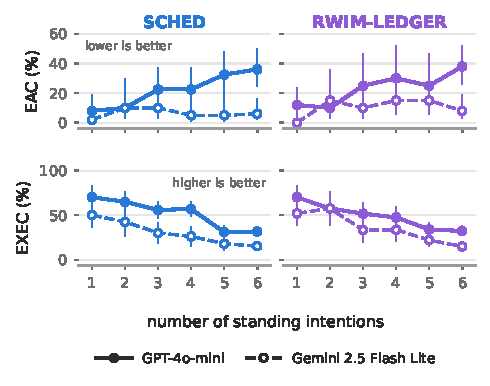
\includegraphics[width=\columnwidth]{fig_load_ledger}
\caption{Load. EAC (top, cancel-early variant) and EXEC (bottom, live
variant: mean share of live intentions carried out) with one to six
standing intentions, under \textsc{sched} (left) and the self-kept
\textsc{rwim-ledger} (right). $n$=50 at one and six intentions, 20 to 40
in between; 95\% intervals. \textsc{bank} at one and six intentions is in
Table~\ref{tab:main}.}
\label{fig:load}
\end{figure}

Execution falls for every actor and design. Of six live intentions the
agents carry out about a third at most (15 to 33\% under \textsc{sched}).
About half of the triggers never come into the agent's view after they
fire; of those that do, the agents act on 60 to 68\% under \textsc{sched}
for three actors and 31\% for Gemini, against 90 to 95\% and 66\% with one
intention.

Whether the rewrite still removes the commission error depends on the
actor. For DeepSeek-V3 and Gemini it does: 7 and 4\% under \textsc{sched}
against 45 and 36\% under \textsc{bank}, with 39 and 33 discordant pairs
against 1, and the self-kept ledger does as well (10 and 7\%). For
Llama-3.3-70B it helps but leaves 18\% against 34\% (18 pairs to 2,
$p=0.0004$). For GPT-4o-mini it is gone: 24 against 32\% (17 pairs to 9,
$p=0.17$), with a correct \textsc{cancelled} entry in view at every step.
Figure~\ref{fig:load} shows where this happens: for GPT-4o-mini the store
degrades from three intentions on, while for Gemini it holds through six,
and execution falls for both. The self-kept ledger follows the same curve
as the harness-kept one at every load, so the loss is not in the
bookkeeping. No design we tested keeps commission low on all four actors,
and none executes more than about a third of the live intentions. This is
the open part of the suite.

\paragraph{Rescheduling.} In a further variant (40 seeds, GPT-4o-mini) the
step-3 message withdraws the intention and gives a new one on another
appliance. The re-injected briefing, which never contains the new
instruction, acts on the withdrawn one in 68\% of episodes and on the new
one in 15\%; the status-tracked store, old entry rewritten and new one
added, in 28 and 50\% ($p\le0.0005$ against the briefing on both); the
self-kept ledger in 15 and 48\%; the rolling summary in 50 and 58\%. No
design handles the update well.
